\chapter{Deployment}
\label{chap:deployment}
% brief introduction into the chapter
In the fast-changing world of web applications, deployment plays a crucial role in the success of any software.
When building a \ac{SaaS} platform meant for various users in various environments, it is important to ensure that the platform is not only adaptable and scalable, but also robust and secure.
This necessity is the foundation on which this chapter is built.
Combining modern cloud technologies with good practices, this section explores how these elements are used in order to ensure smooth and efficient deployment process.
With a focus on \ac{IaC}, this chapter highlights how this method is used within the \ac{AWS} ecosystem providing in-depth look at the deployment procedure for both frontend and backend components discovering how they directly impact scalability, reliability, and security of the platform.

\section{Current Deployment Strategy}
\label{sec:current-deployment-strategy}
%  introduce the current deployment strategy of project
%  the deployment is managed using Infrastructure as Code (IaC) on AWS, use of specific services (Amazon S3 for hosting the static frontend and AWS Lambda for the backend functionality)
% how these components are organized into multiple stacks using AWS cloudformation

The deployment strategy for this projects leverages \ac{AWS} services with focus on \ac{IaC} to automate and manage cloud infrastructure.
Thanks to this approach, creating a consistent deployment process is achieved while reducing possibilities of human error and ensuring replication across different stages or environments.

Specifically, the strategy uses Amazon \ac{S3} for hosting the static frontend(s), \ac{AWS} Lambda for backend functionalities including scheduled background tasks and organising these diverse components into multiple stacks using \ac{AWS} CloudFormation.
Furthermore, this project improves its architecture with the inclusion of the PostgreSQL database using \ac{RDS}, Amazon Route 53 for domain routing, Amazon Certificate Manager for SSL/TLS certificate management and Amazon \ac{SES} for securing a high email delivery rate.
This structure allows for a well-controlled infrastructure, allowing quick adjustments if needed.

\subsection{Amazon Simple Storage Service for Static Frontend Hosting}
\label{subsec:amazon-s3-static-frontend}
% how Amazon S3 is used for storing and serving the static ReactJS app
Deploying static frontend applications of the platform employs the Amazon \ac{S3} to host the ReactJS applications. Amazon \ac{S3} provides a reliable, scalable and secure solution for serving static content, making it ideal choice for hosting a \ac{SPA} applications like ours.
All three frontend applications (documentation, tracking page and dashboard) use very similar deployment strategies.
The \ac{S3} buckets are configured to serve a website with \texttt{index.html} with allowing public access and establish removal policies to ensure that the buckets are destroyed when needed. 
However, we cannot provide access to the \ac{S3} bucket just like that.
The definition of Amazon CloudFront distribution (Amazon \ac{CDN}) is vital to catch errors and unauthorised accesses by enforcing a \ac{SSL} certificate managed by \ac{AWS} Certificate Manager.
Finally, \ac{DNS} routing for applications is configured with Amazon Route 53, creating an A record that points to the CloudFront distribution.
For a detailed visualisation of the deployment architecture for static frontend applications and how these components connect, refer to the diagram illustrated in \ref{img06:fig_static-webapp} 


\begin{figure}[p]\centering
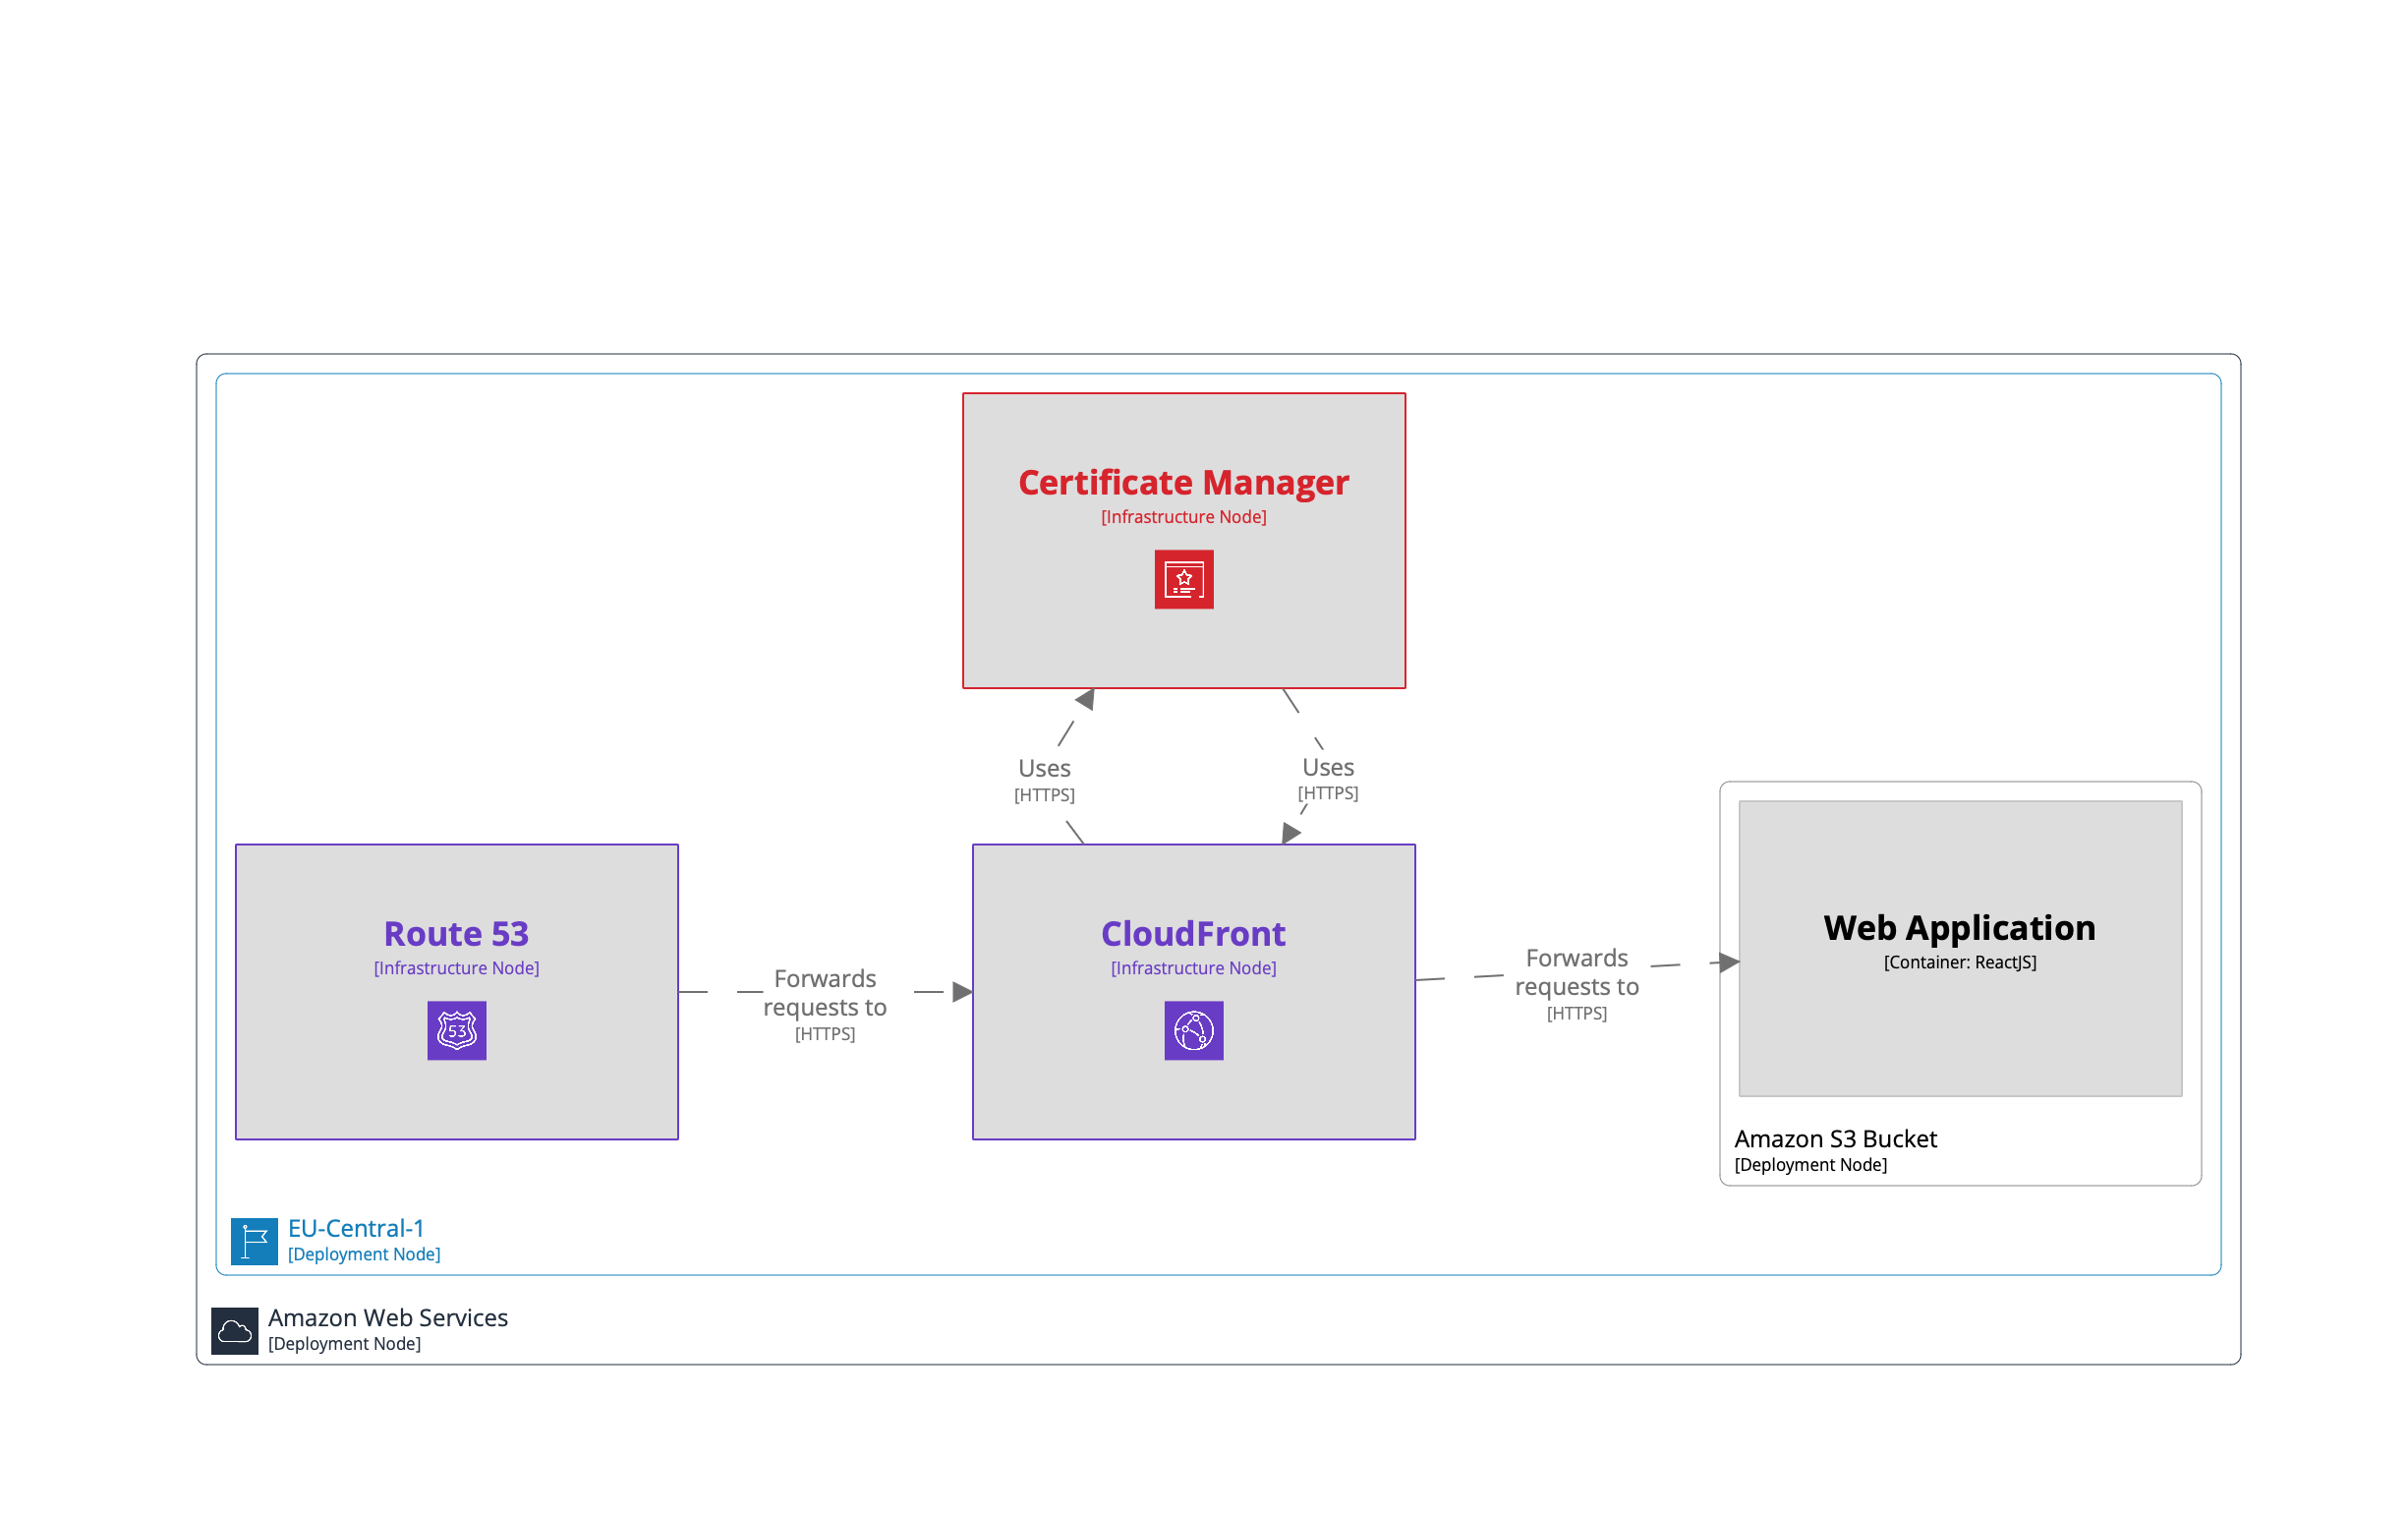
\includegraphics[width=140mm]{img/chap06/fig_static-webapp.png}
\caption{C4 Deployment diagram of static web application in AWS}
\label{img06:fig_static-webapp}
\end{figure}

\subsection{AWS Lambda for Backend Services}
\label{subsec:aws-lambda-backend}
% use of AWS Lambda for the backend
% discussing how serverless architecture benefits the application, including scalability, cost-efficiency, and reduced operational overhead.
For the backend services, the project leverages \ac{AWS} Lambda, a serverless computing service that runs code in response to events with automatic management of underlying computing resources.
This choice supports a serverless architecture for the backend, benefiting from scalability of Lambda functions, which scale automatically based on the number of requests and are quite cost-efficient by charging only for the compute time consumed.
Such a pricing strategy is important for our platform, primarily operational during the Central European working hours, ensuring that resource allocation during off-peak hours - such as nights, early morning and weekends - is minimized, thus aligning resource usage with the actual demand.

The entire \texttt{KoaJS} backend is encapsulated within Lambda functions using the \texttt{Serverless} framework. 
This setup not only streamlines the deployment and operation of the serverless backend, but also enhances its extensibility and maintainability.
The \texttt{Serveless} framework handles the integration of backend application into the \ac{AWS} ecosystem, enabling leveraging the full spectrum of benefits of serverless computing.

Additionally, the backend is expanded with serveral scheduled tasks, configured to emulate traditional cron jobs within the Lambda environment.
These tasks are crucial for routine operations such as fetching parcel statuses from carrier APIs and sending tracking emails to recipients.
Specific Lambda handles are designed for database seeding and migrations tasks which are crucial for the deployment process.
These handlers are invoked as part of the \ac{CI}/\ac{CD}.

The \ac{IaC} approach for the deployment of the backend service is orchestrated thought \texttt{AWS CDK}, enabling automated provisioning of cloud resources.
Key elements of the deployment include the following:
\begin{itemize}
    \item \textbf{AWS Lambda:} The main building block of the backend service, AWS Lambda functions are integrated to run code in response events.
    \item \textbf{Data storage and management:} A PostgreSQL hosted on Amazon \ac{RDS} provides a managed, scalable and secure relation database solution that accompanies automated tasks such as backups and patching.
    \item \textbf{Network configuration:} A dedicated \ac{VPC} is provisioned to encapsulate Lambda functions, ensuring that they operate within a secure and isolated network environment. Security groups within \ac{ VPC} define access rules, providing a security layer for backend interactions.
    \item \textbf{API Gateway integration:} An API Gateway acts as the entry door backend services, managing incoming API requests and routing them to the appropriate Lambda function.
    \item \textbf{Domain management and \ac{SSL}/\ac{TLS} encryption:} The deployment also uses Amazon Route 53 for domain routing and \ac{AWS} Certificate Manager to manage \ac{SSL}/\ac{TLS} certificates. 
    \item \textbf{Static content hosting}: Amazon \ac{S3} buckets are integrated to host static assets used for user-uploaded public content.
\end{itemize}

For a more in-depth look, refer to the diagram illustrated in \ref{img06:fig_lambda}

\begin{figure}[p]\centering
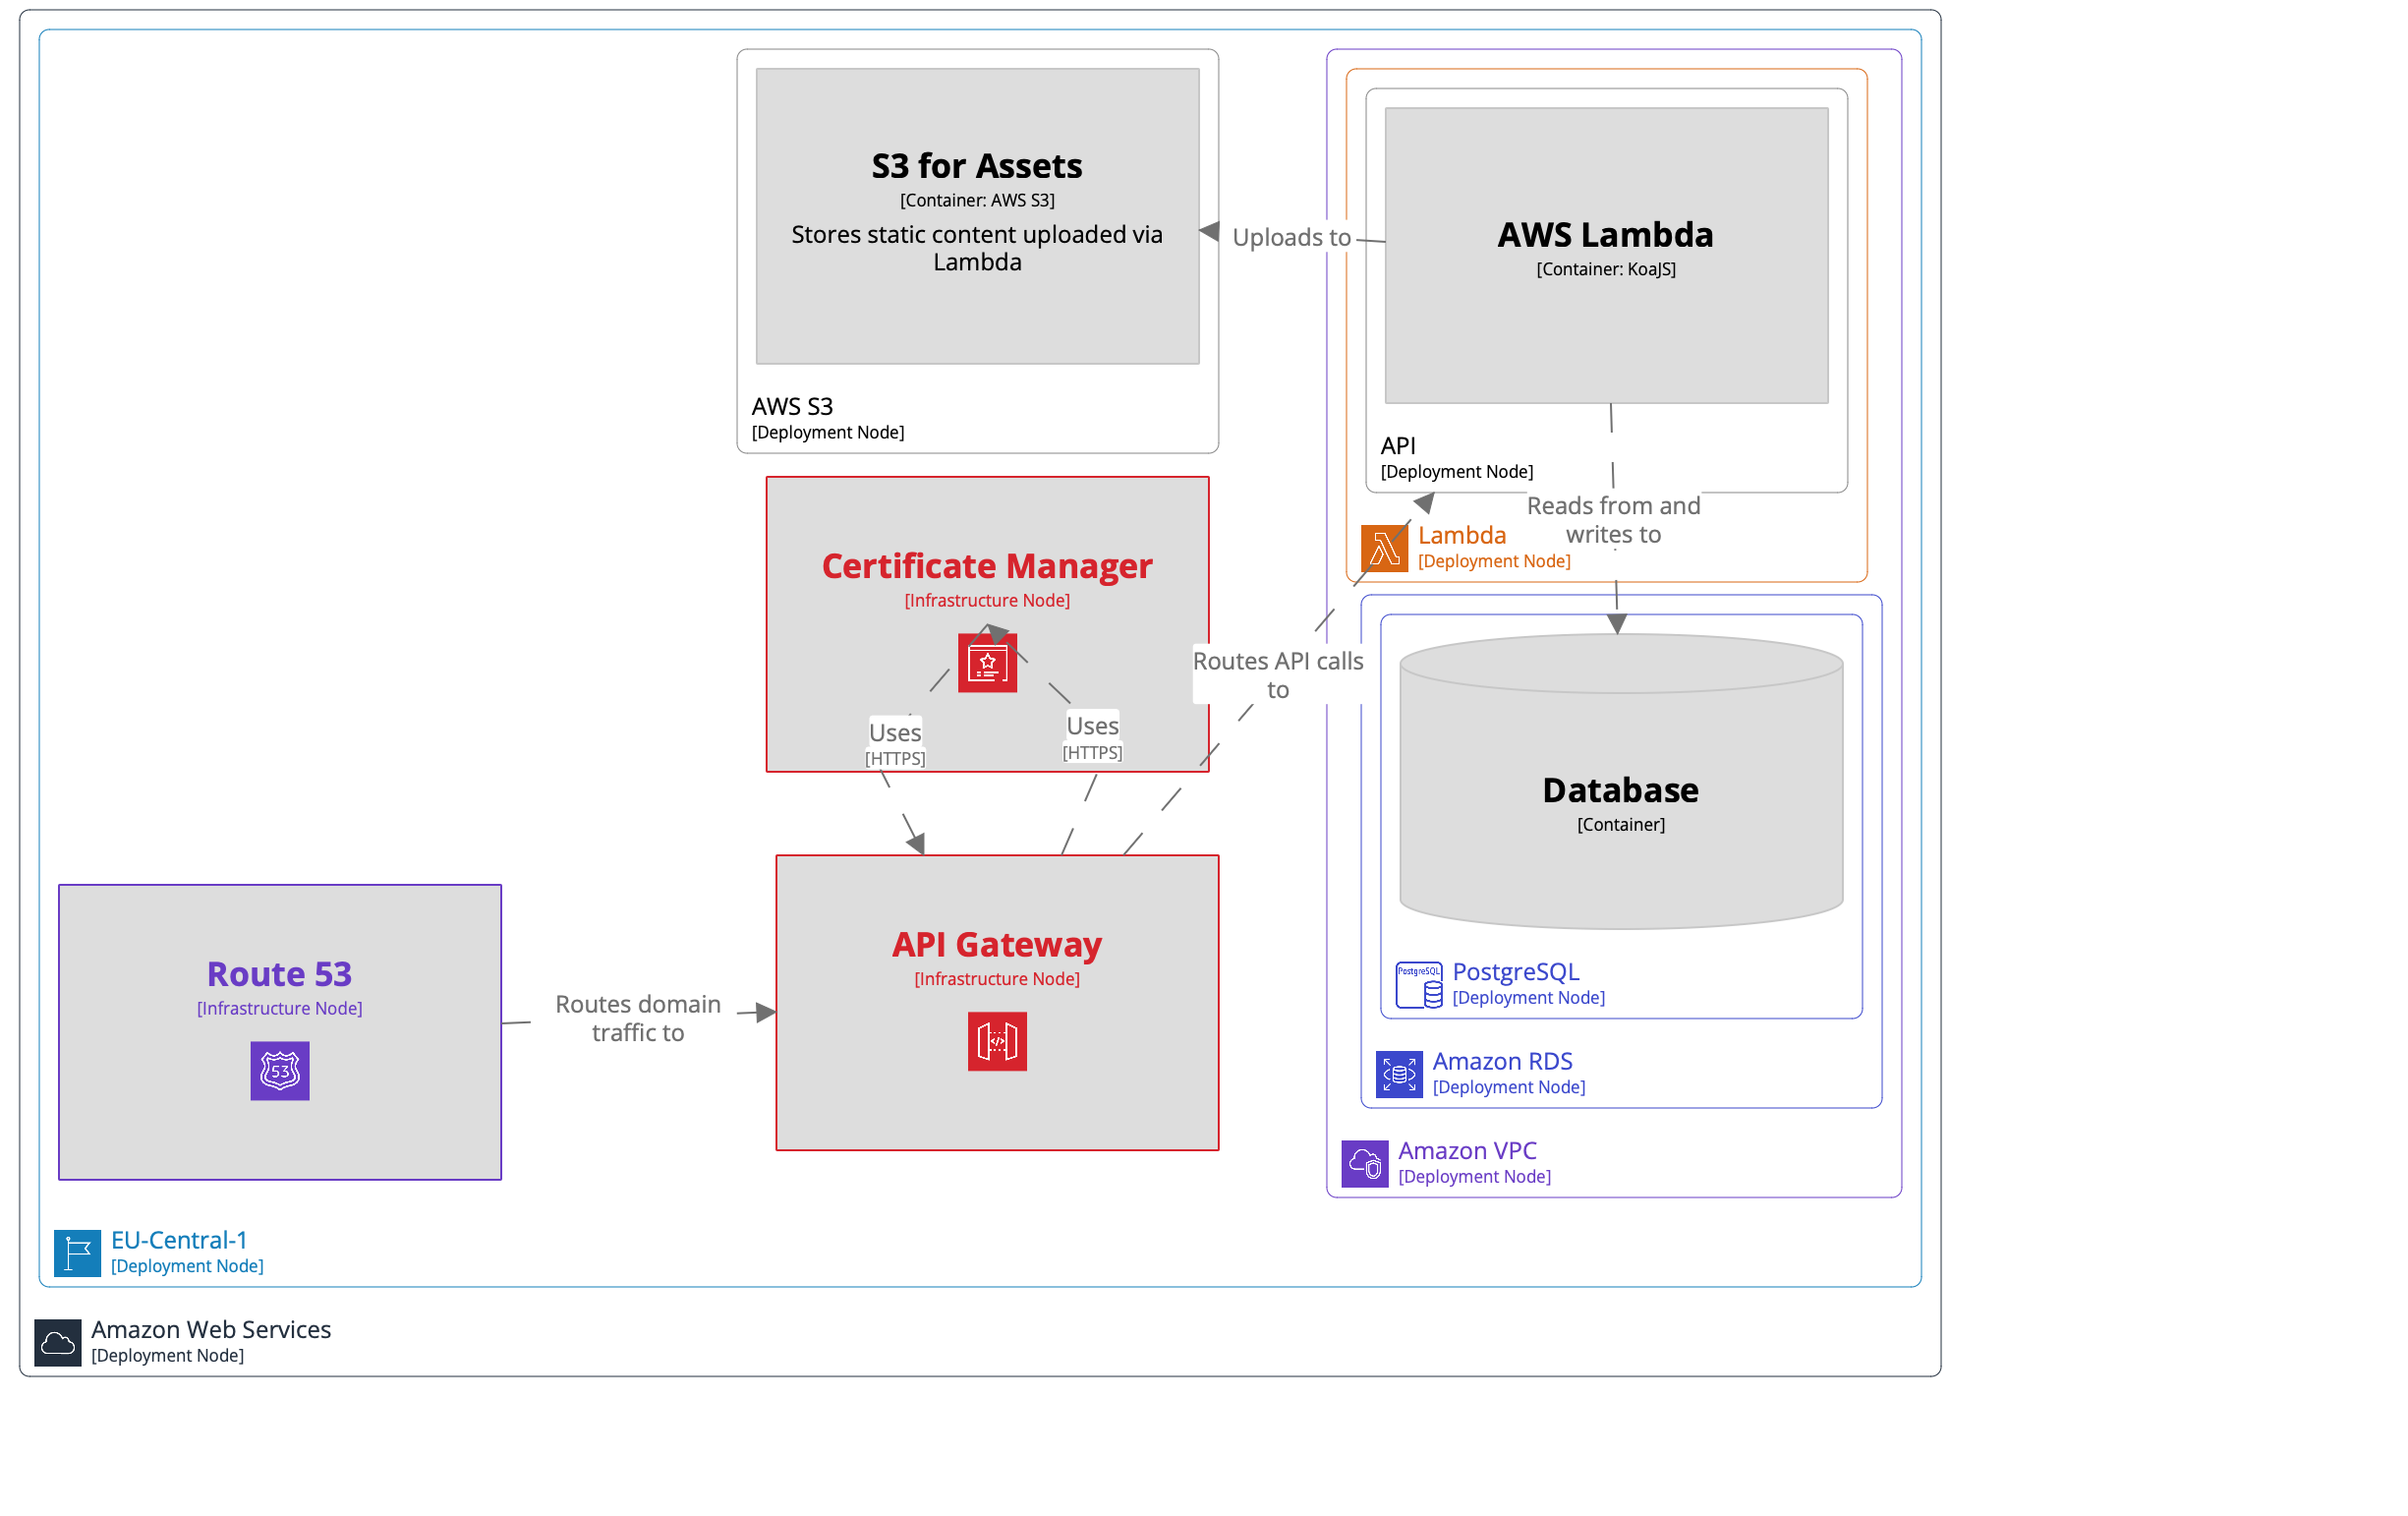
\includegraphics[width=140mm]{img/chap06/fig_lambda.png}
\caption{C4 Deployment diagram of backend service in AWS}
\label{img06:fig_lambda}
\end{figure}


\subsection{AWS CloudFormation for Infrastructure Management}
\label{subsec:aws-cloudformation-infrastructure}
% the role of AWS cloudformation in managing the infrastructure.
% consistent, repeatable deployment processes

\ac{AWS} CloudFormation plays a crucial role in managing the project infrastructure.
It perfectly aligns with the purpose of \ac{IaC} - to create and manage resources with templates.
CloudFormation enables the user to define the entire cloud environment as code that can be versioned, reused, and shared. 
Automating the deployment of resources in a consistent and repeatable manner.
By organising resources into multiple stacks, the deployment can be segmented logically (e.g., networking, application layers, security), facilitating easier management and updates of specific components.
Using the \ac{AWS} CloudFormation, one can define the \ac{IAM} roles and policies that define the permissions and actions that can be performed on \ac{AWS} resources.
This policy is a key factor in reducing the scope of operations for the deployment process, ensuring that each action, from the deployment of Lambda functions to the management of log groups and the interaction with other services like \ac{S3} and \ac{RDS}, is guided by a set of permissions. 

In our case, several CloudFormation stacks are created using \ac{AWS CDK} to programmatically define and manage CloudFromation stacks.
As a result, the deployment process systematically manages the creation of several key CloudFormation stacks, each designed to support different facets of the application's infrastructure:
Having said that the deployment creates the following CloudFormation stacks:
\begin{itemize}
    \item \textbf{API Service Stack:} Central backend infrastructure, the API Service Stack comprises all the necessary resources deployed by the \texttt{Serverless} framework such as all Lambda handlers and events triggering the scheduled tasks.
    \item \textbf{Docs page stack:} Dedicated to the application documentation portal, the Docs page stack provides the infrastructure required to host and serve the documentation. 
    \item \textbf{Tracking page stack:} Tailored for the tracking functionality, this stack establishes the infrastructure needed for the tracking page.
    \item \textbf{Dashboard page stack:}  Focused on the administrative aspect of the application, the Dashboard Page Stack creates the infrastructure for the dashboard page. 
\end{itemize}

\section{Alternative Deployment Methods}
\label{sec:alternative-deployment-methods}
% This section should explore alternative deployment methods that could be used for the project.

While the chosen deployment path for this project is \ac{AWS} with serverless architecture for deployment, it is important to explore alternative deployment methods that might offer different benefits or better align with specific needs.
Two main alternatives are containerisation and utilisation of services from other cloud providers.


\subsection{Containerization}
\label{subsec:containerization}
% concept of containerization, particularly using Docker
% how containerization could be applied to both the frontend and backend
Containerization is a method that allows to encapsulate an application along with its environment and dependencies into a container that should run consistently on any infrastructure. 
Being either a local development environment or production on a remote server, containers are increasing in popularity and are very often the way to go for both development and deployment.
This approach is complemented by technologies such as Docker.
Docker can run completely free in both development and production environments, significantly reducing cost.
This gives freedom to the deployment environment. 
Containers can run on a bare \ac{VPS} or in a container-specific environment developed to host containers without taking the costs of maintaining a server such as Amazon \ac{ECS}.
 Containerisation offers numerous benefits, including:
 \begin{itemize}
     \item \textbf{Portability:} Containers can be moved across different environments or cloud providers without vendor-lock-in.
     \item \textbf{Efficiency:} Containers share the kernel of the host system, making them more lightweight and efficient than running separate \ac{VPS} for each application.
 \end{itemize}


\subsection{Other Cloud Providers and Services}
\label{subsec:other-cloud-providers}
% Briefly touching on alternative cloud providers (like Azure or Google Cloud Platform) and their services that could be used for a similar deployment strategy.
In today's world, choosing between cloud providers is not a simple task.
One can choose between more abstract solutions (cloud platform as a service) that require less setup, hiding more complexity behind.
This usually comes with some costs that are either financial or functional.
The reason being is that these platforms usually run on outsourced hardware and that they should be widely accessible by application developers without expertise in deployment and server problematic. 
This is so because making processes simpler usually requires significant reductions in the configuration options and settings. 
A good example might be a Vercel, a cloud platform as a service company providing a simple to use solution to host web applications.
However, for us, a more complex solution was needed. 

\subsubsection{Google Cloud Platform (GCP)}
\ac{GKE} offers powerful and scalable container deployment solution.
Google Cloud Run is a fully managed platform that automatically scales containers, similar to AWS Lambda but with the benefits of containerisation. 

\subsubsection{Microsoft Azure}
Microsoft's \ac{AKS} might provide a similar solution to \ac{GKE}. However, using Azure Functions, which supports serverless computing, might be a better match to \ac{AWS} Lambda, which supports an event-driven environment.

\subsection{Conclusion}
Although the current deployment strategy uses \ac{AWS} services and a serverless architecture that offers good scalability, exploring alternative deployment methods such as containerisation presents an opportunity to minimise the potential risks associated with vendor lock-in.

Vendor lock-in occurs when a project becomes so dependent on a particular cloud provider that migrating is technically challenging or expensive.
However, the benefits of avoiding vendor lock-in must be balanced against the complexity of deployment and infrastructure management.
If one wants to handle secure and scalable deployment following recommended practices on a bare metal without vendor lock-in, it becomes a very challenging task.



\section{Continuous Integration and Continuous Deployment (CI/CD)}
\label{sec:cicd}
% Dedicate this section to the CI/CD processes implemented in the project, emphasizing the use of GitHub Actions.
In every project, both \ac{CI} and \ac{CD} processes are crutial components to ensure code quality and minimize possible human error on repetitive manual task such as deployment.
Using GitHub Actions as the running environment of the \ac{CI}/\ac{CD} pipeline allows the automation of various workflows ranging from code quality checks to deployment into two separate environments (staging and production), ensuring that every line of code in the \texttt{main} branch of the code repository undergoes through lint and build checks with follow-up deployment.

\subsection{GitHub Actions for CI/CD}
\label{subsec:github-actions-cicd}
% how GitHub Actions are used for CI/CD
% details on how code changes in the repository trigger automated workflows for building, and deploying both the frontend and backend components

Since GitHub was chosen as the primarily code repository for the project, it was a straightforward choice to use cloud runners in GitHub Actions as the go-to solution for the integration and deployment pipeline.
When code changes in the repository, GitHub Actions are triggered to execute predefined jobs, such as typing checks with \texttt{TypeScript}, linting with \texttt{ESLint}, and the identification of spelling errors.
These initial steps ensure that the code base adheres to the project's standards and conventions.

Following quality checks, deployment workflows are activated based on pushing to the \texttt{main} branch publishing the code to both production and staging environments with all necessary migrations and updates.
These workflows use \ac{AWS CDK} commands and \ac{AWS CLI} to deploy infrastructure changes and application updates to \ac{AWS} services, effectively and relatively quickly, bringing the application from the repository to the world.


\subsection{Workflow Automation and Pipeline}
\label{subsec:workflow-automation-pipeline}
% specific steps involved in  CICD pipeline, including code commits, automated testing, build processes, and deployment to AWS services.
The integration and deployment pipeline is designed to ensure consistent code style with minimizing propagation of errors into the public production environment.
The phases of the pipeline are the following.
\begin{itemize}
    \item \textbf{Code quality checks:} On every pull request, automated workflow for linting, type checking and spelling is triggered. These steps are important for maintaing high code quality and catching potential issues early.
    \item \textbf{Build process:} For frontend applications, the build process compiles the source code into static assets. Backend services are prepared for deployment, ensuring that all necessary dependencies are correctly packaged.
    \item \textbf{Deployment to AWS services:} Deployment is carried out in stages, starting from staging to production environments. If something fails, the staging process is over, production is terminated, and the job fails. This phased approach allows for validation of changes in a controlled context before affecting live users. \ac{AWS CDK} is used to provision or update \ac{AWS} resources, including Lambda functions for backend services and \ac{S3} buckets for hosting frontend assets. Infrastructure changes are managed through CloudFormation stacks, allowing for reliable and repeatable deployments.
    \item \textbf{Post-Deployment tasks:} After the build and deployment, database migrations and invalidating CDN caches ensure that the latest and valid content is served to user and that the database schema is up to date with what application is expecting.
\end{itemize}

By integrating these steps into GitHub Actions, the project benefits from an automated pipeline minimising manual intervention in error-prone processes.
For example, on the \ref{img06:fig_github_actions_integration} are three stages of the code quality pipeline.
\begin{figure}[p]\centering
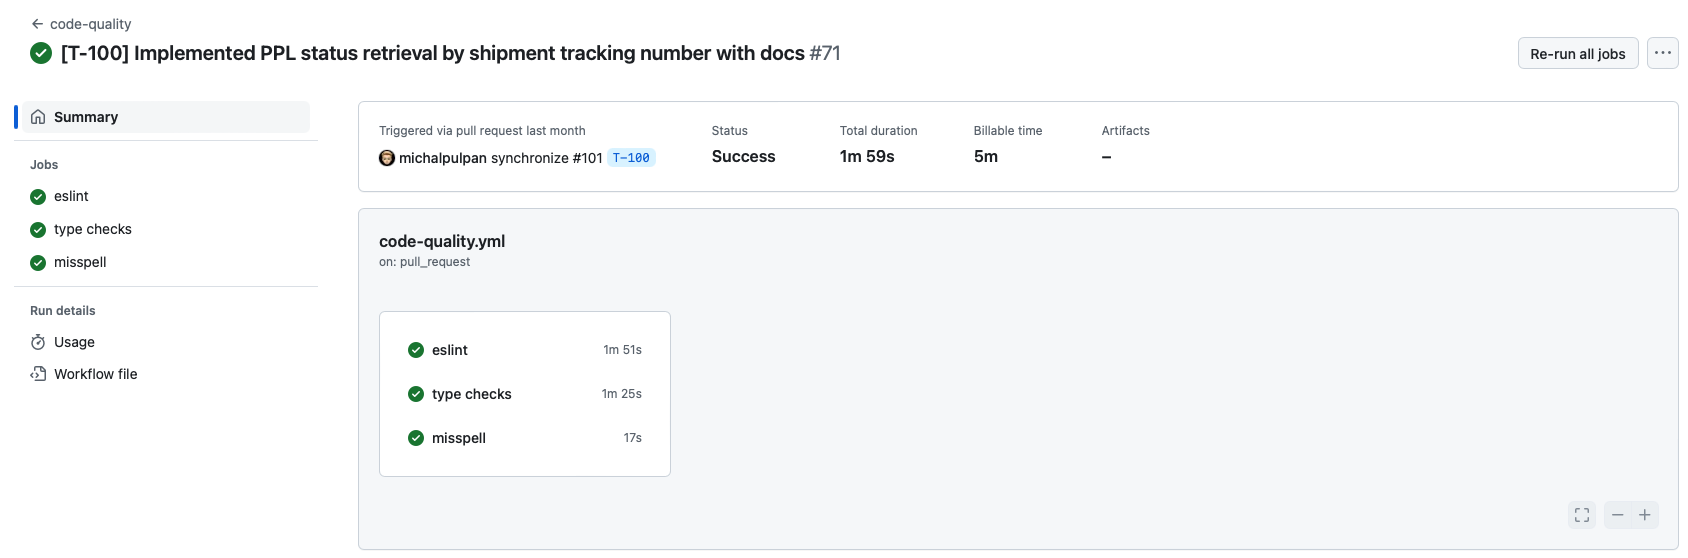
\includegraphics[width=140mm]{img/chap06/fig_github_actions_integration.png}
\caption{GitHub Actions - Pull request integration}
\label{img06:fig_github_actions_integration}
\end{figure}
On the other hand, on \ref{img06:fig_github_actions_deployment} we can see two phase deployment process firstly into staging environment with follow-up production for all components of the platform. For a detailed view, we can see \ref{img06:fig_github_actions_api_deployment} where all the steps of the API production deployment can be seen.

\begin{figure}[p]\centering
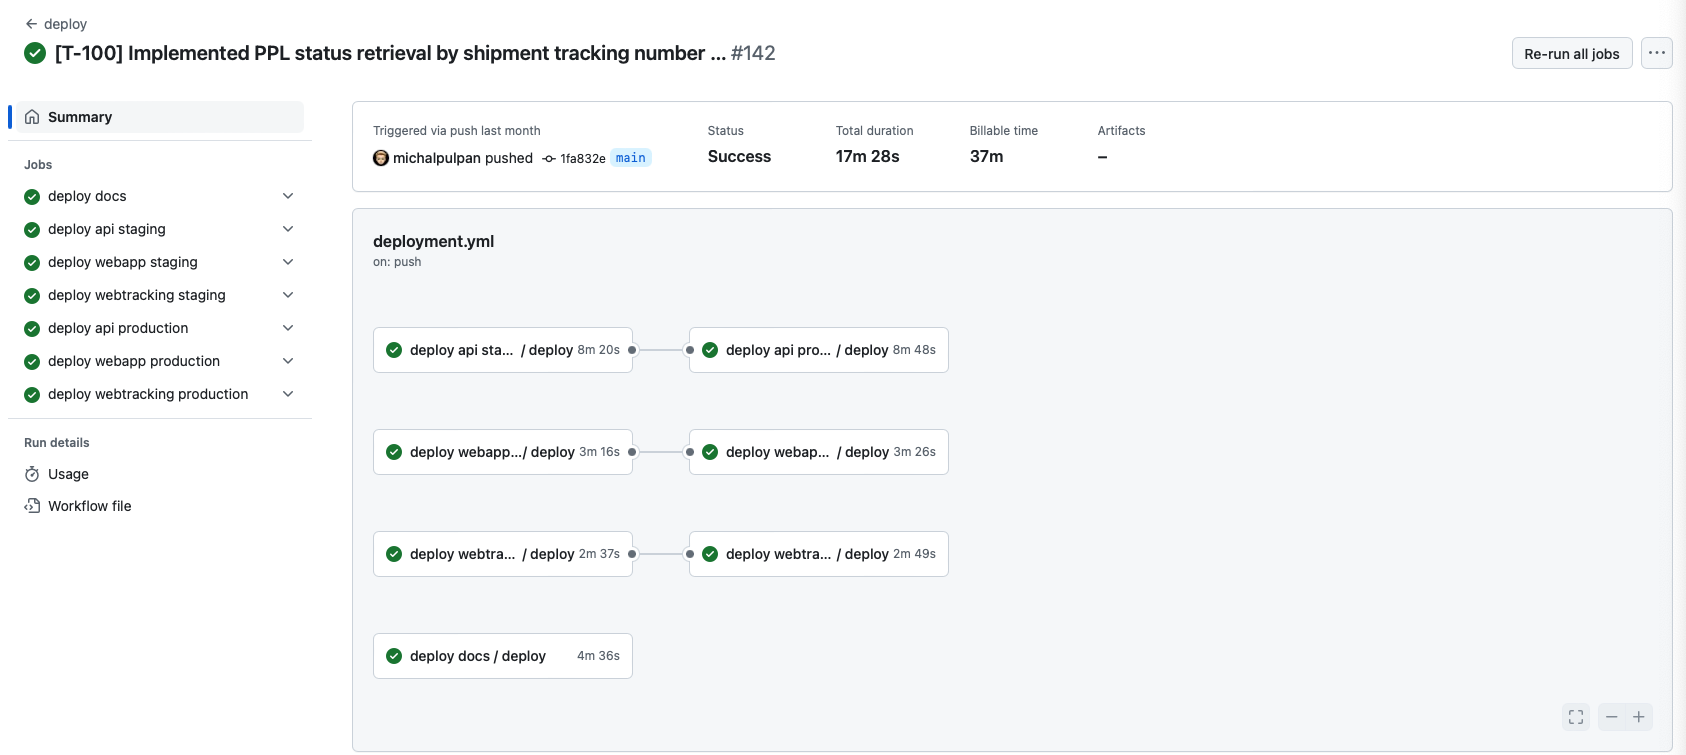
\includegraphics[width=140mm]{img/chap06/fig_github_actions_deployment.png}
\caption{GitHub Actions - merge deployment}
\label{img06:fig_github_actions_deployment}
\end{figure}
\begin{figure}[p]\centering
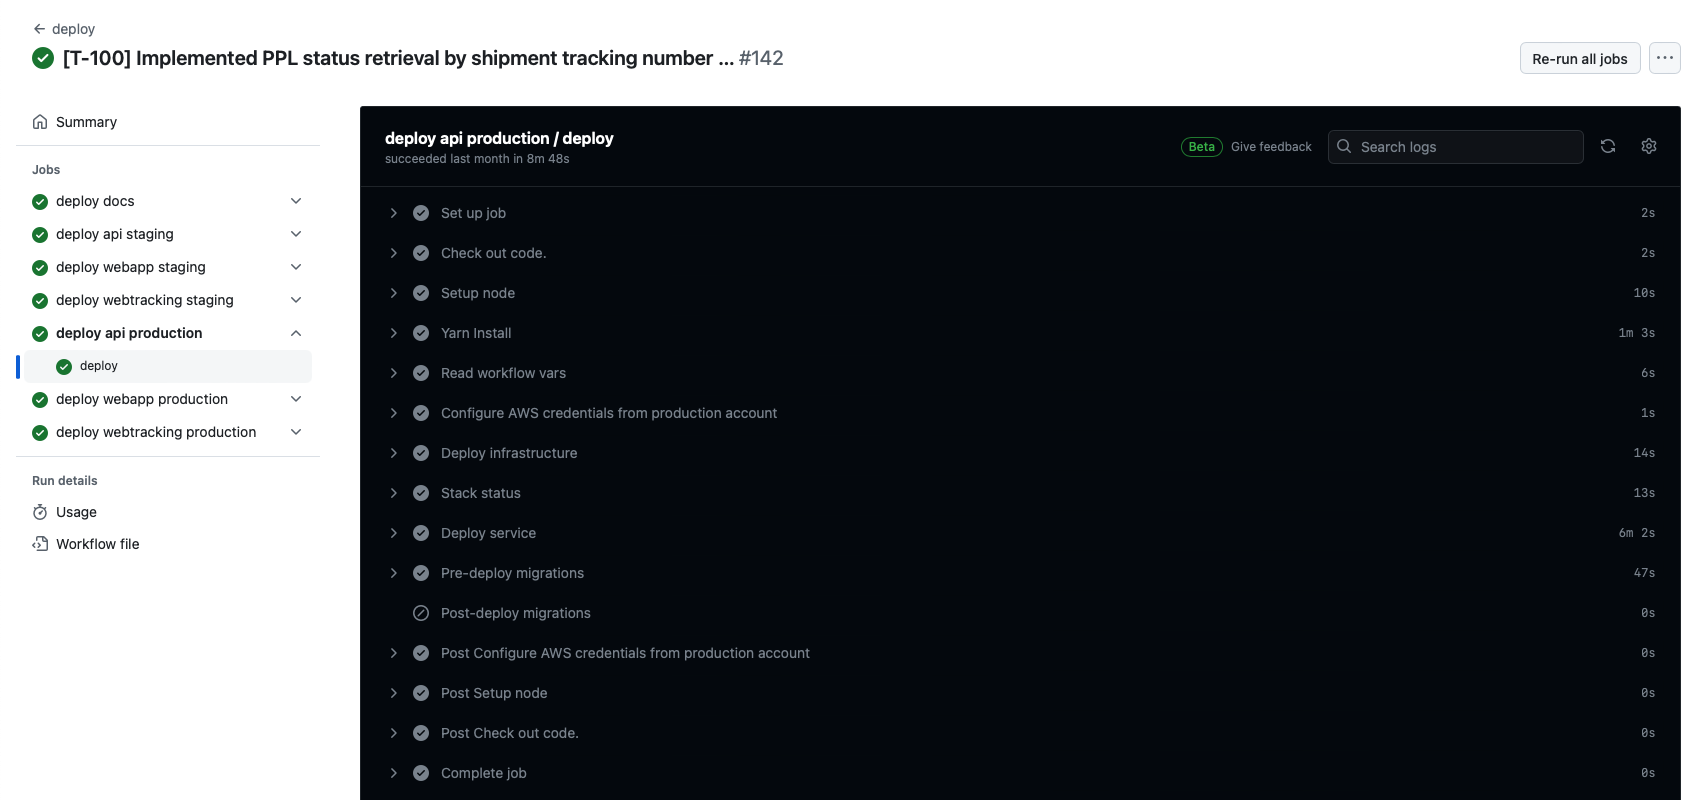
\includegraphics[width=140mm]{img/chap06/fig_github_actions_api_deployment.png}
\caption{GitHub Actions - merge deployment API}
\label{img06:fig_github_actions_api_deployment}
\end{figure}

This significantly speeds up the deployment cycle and ensures better stability of the application.




